% !TEX root = ../my-thesis.tex
%
\chapter{Pipeline}
\label{sec:pipeline}

\section{Pipeline overview}
\label{sec:pipelineoverview}

\begin{figure}[htb]
	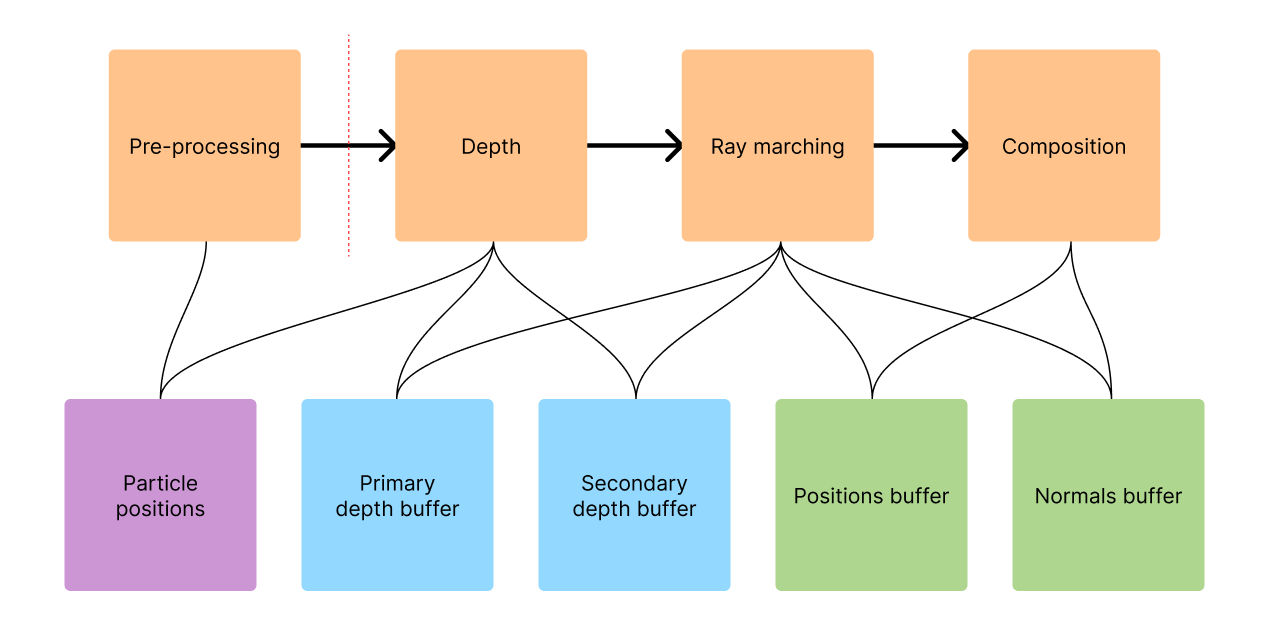
\includegraphics[width=\textwidth]{my-gfx/figure-pipeline.png}
	\caption{The computation pipeline and data flow of the program. The passes of the pipeline are displayed in orange. Regarding the data structures at the bottom: arrays are purple, depth buffers are blue, and color buffers are green. Pre-processing is decoupled in our implementation but can be incorporated into the per-frame computations.}
	\label{fig:pipelineoverview:pipeline}
\end{figure}

In this chapter, we show a high-level overview of the pipeline that all data flows through to eventually create an image on the screen. We aim to provide context for the following chapters that go more deeply into explaining the authors' work.

The proposed algorithm works through multiple passes, each one taking the output of the previous one as input. The input to the entire pipeline is an array of three-dimensional particle positions that represent the fluid at one particular moment in time. In Figure \myref{fig:pipelineoverview:pipeline}, we illustrate which part of the pipeline accesses which data structures.

\subsection{Pre-processing}

During this pass, the particle data is pre-processed and acceleration structures are built that serve the purpose of speeding up the following passes. An important note is that Wu et al. incorporate this pass into their algorithm tightly. It is executed in every frame of the visualization by processing it on the GPU. We on the other hand decided to run it only once when loading the dataset as it is the most time-consuming part of our implementation. We provide more information on how to improve on this in the chapter \textbf{Future work \myref{sec:futurework}}.

Firstly, the so-called \textit{binary density grid} (also called \textit{density mask} in the paper) is generated (Wu et al. \cite{Wu:2022}, section 4.1). Space is divided into a grid of cells. Each cell holds a boolean value indicating whether it is at all possible for the algorithm to find the fluid's surface inside the cell. For that, the maximum density of the fluid is approximated. If it does not exceed a certain threshold, the cell can safely be skipped to save valuable computation time.

Secondly, each particle is classified as either belonging to a dense ("\textit{aggregated}") or to a sparse part of the fluid (splashes). This information is used in the depth pass when deciding which depth buffer the particle should be rendered to (more in the chapter \textbf{Handling splash particles \myref{sec:splashparticles}}).

\subsection{Depth pass}

In the depth pass, particles are rendered to a depth buffer as spheres with the radius $h$. The positions on those spheres serve as good approximations of the true fluid surface. They are used as starting points for refinement during the ray marching pass.

Two depth buffers are filled during this pass. The authors call these $D$ and $D_{agg}$, we call them the primary and secondary depth buffer respectively. All particles are rendered to the primary buffer, but only the ones classified as "aggregated" are rendered to the secondary buffer. More information on this is provided in the sections \myref{sec:depth} and \myref{sec:splashparticles}.

\subsection{Ray marching pass}

Rays are shot from the camera into the scene along which the fluid surface is searched. The depth buffer from the previous pass is used to compute entry points for the rays (more in the chapter \textbf{Surface extraction with ray marching \myref{sec:surfaceextraction}}). Since this pass is very costly on its own,  the authors provide several adaptive techniques for reducing the time spent ray marching - for example a hash grid and variable resolution.

\subsection{Composition pass}

The last step of the pipeline is to take the data computed in all previous passes and determine a color for each pixel of the screen. Here, the fluid's properties like color, refraction, transparency, and light interaction are modelled and it is embedded into the scene (more in the chapter \textbf{Image composition \myref{sec:imagecomposition}}).

\section{Depth pass}
\label{sec:depth}

\begin{figure*}[h]
    \centering
    \begin{subfigure}[b]{0.475\textwidth}
        \centering
        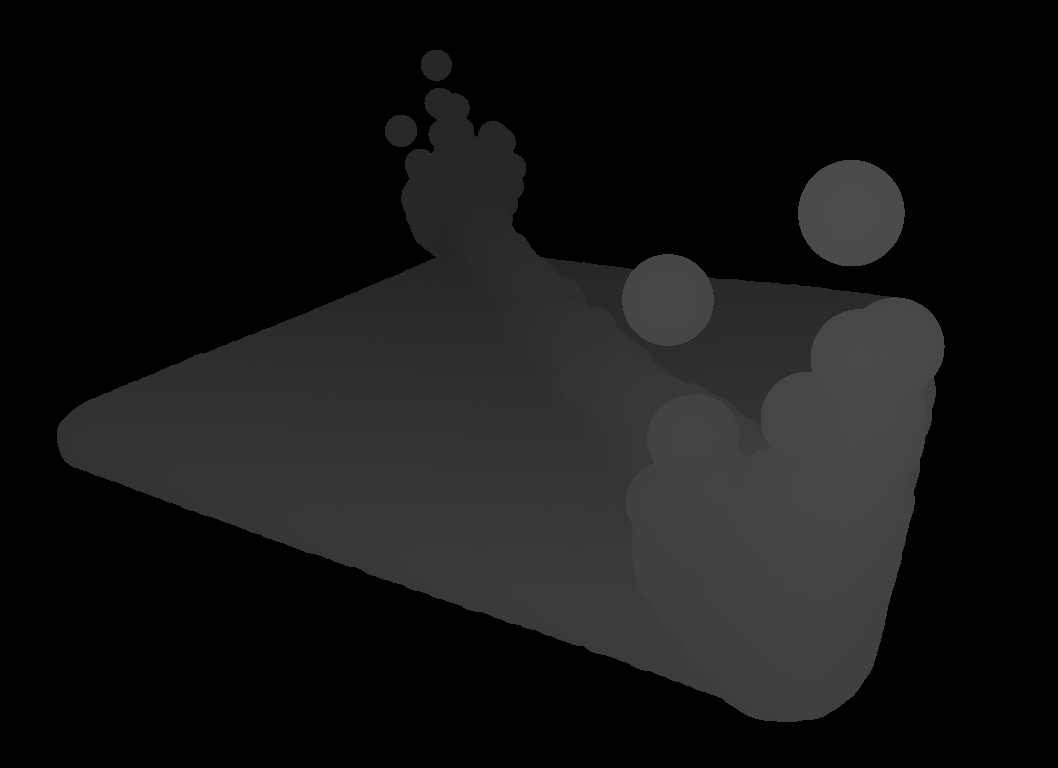
\includegraphics[width=\textwidth]{my-gfx/figure-depth-buffer-1.png}
    \end{subfigure}
    \hfill
    \begin{subfigure}[b]{0.475\textwidth}  
        \centering 
        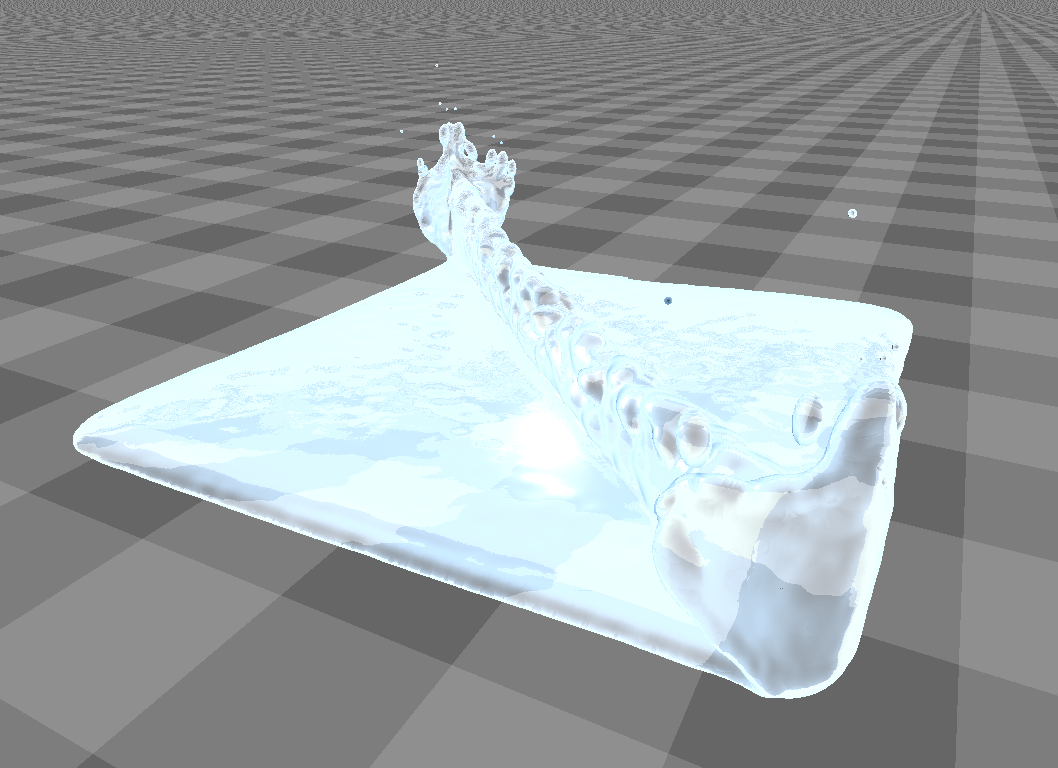
\includegraphics[width=\textwidth]{my-gfx/figure-depth-buffer-2.png}
    \end{subfigure}
    \vskip\baselineskip
    
    \caption{\textit{Left}: The depth buffer of a visualization frame (inverted). Particles appear as smooth spheres. Lighter areas are closer to the camera. \textit{Right}: The resulting image after the composition pass.}
    
    \label{fig:depthbuffer}
\end{figure*}

\begin{figure}[h]
    \centering
    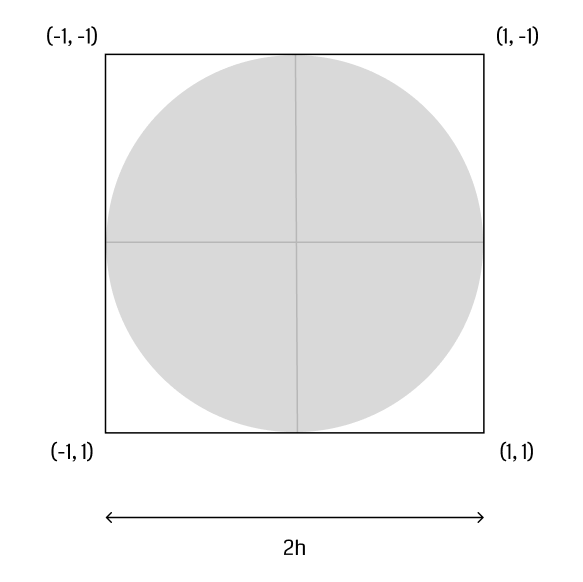
\includegraphics[width=0.5\textwidth]{my-gfx/figure-uvs.png}
    \caption{A quad of two triangles representing one particle. The texture coordinates are set up for computing a spherical offset in the z-direction}
    \label{fig:depth:uvs}
\end{figure}

After pre-processing has taken place, the particles are rendered into depth buffers that serve as entry points for the surface reconstruction (see Figure \myref{fig:depthbuffer} for a visualization of a depth buffer).

The first step is to construct a vertex buffer that holds all particles comprising the fluid. Wu et al. suggest to render a camera-facing quad for each particle with sidelength $2h$. Each vertex holds
\begin{enumerate}
    \item a three-dimensional position in world space,
    \item and a two-dimensional texture coordinate - $(-1, -1)$ for the top left, $(1, 1)$ for the bottom right vertex (Figure \myref{fig:depth:uvs}).
\end{enumerate}
The vertex buffer is fed into the first render pass, which writes to the depth buffers. The value output to the buffer is:
\[ depth := z - \cos(\frac{\pi}{2} r) \]
with $r := \sqrt{u^2 + v^2}$ being the world-space distance from the particle's center and $z$ being the particle's z-coordinate. The fragment is discarded if $r > 1$.

This technique renders the particles as if they were perfect spheres - although they are rendered simply as two triangles - by projecting onto the surface of the camera-facing hemispheres surrounding the particles. Conveniently, by using a depth buffer for this pass, occlusion is handled efficiently by the graphics hardware.

Two depth buffers will be filled using this technique:
\begin{enumerate}
    \item the \textit{primary} depth buffer (called $D$ in the paper) containing all particles
    \item and the \textit{secondary} depth buffer (called $D_{agg}$ in the paper) containing only particles belonging to a denser ("aggregated") part of the fluid volume.
\end{enumerate}
The former will be used as a first estimation of the fluid's surface. The latter will be used to enable the ray marcher to skip large parts of empty space and continue at the surface again (further details in chapter \textbf{Methods of acceleration \myref{sec:acceleration}}).


\section{Surface extraction with ray marching}
\label{sec:surfaceextraction}

Ray marching has gained popularity in recent years as a surface extraction method for particle-based representations as it suits the parallel nature of computation on GPUs. It can be implemented in a compute or fragment shader and executed independently. Although this is the way the authors designed their implementation, we had to refrain from following that path for lack of time. This step, however, would lead to significant reductions in computation time.

Ray marching refers to a technique of sampling some function at points along a ray and collecting information about the function in the process. In our application, we shoot rays from the camera to sample the fluid's density $\rho$ and find a point where the surface criterion is met (see the surface definition \myref{sec:surfacedefinition}). Theoretically - since the fluid is continuous -, infinitely many rays would be needed to capture the entire surface. For graphical applications, however, the finest granularity of information can be retrieved at the pixel level. Any surface information between pixels would not - at least not in the algorithm discussed here - contribute to the final image. Hence, all the following computations are performed for each pixel of the screen (of size $WIDTH \times HEIGHT$) labeled $i$.

In mathematical terms, we search for a point $\textbf{r}$ along the ray
\[ \textbf{r} = \textbf{a} + t \textbf{v}, \space t \in [0, \infty) \]
where the following condition is satisfied:
\[ \rho ( \textbf{r} ) = \sigma. \]
In the ray equation, $\textbf{a}$ is the starting position of the ray and $\textbf{v}$ is a unit-vector indicating the direction the ray is travelling in. They can be computed by applying the inverse transformation pipeline ($\textbf{P}$ being the projection and $\textbf{V}$ being the camera matrix) to the homogenous clip space coordinates $( x, y, z, 1 )^T$:
\[
\tilde{\textbf{a}} :=
\begin{pmatrix}
\tilde{\textbf{a}}_x \\
\tilde{\textbf{a}}_y \\
\tilde{\textbf{a}}_z \\
\tilde{\textbf{a}}_w
\end{pmatrix} =
\textbf{V}^{-1} \space \textbf{P}^{-1} \space
\begin{pmatrix} x \\ y \\ z \\ 1 \end{pmatrix}
\]
$z \in [0, 1]$ is looked up directly from the primary depth buffer. If $z = 1$, the depth pass did not output a value for this pixel, meaning there is no fluid surface to be found. In this case, the pixel can be discarded. $x, y \in [-1, 1]$ are retrieved with the following computations. The pixel coordinates are converted to so-called normalized device coordinates:
\[ x := 2 \frac{i \text{ mod } WIDTH + 0.5}{WIDTH} - 1 \]
\[ y := 2 \frac{\lfloor i / WIDTH \rfloor + 0.5}{HEIGHT} - 1 \]
where $i$ is the index of the current pixel counting row-wise from the origin of the screen. The origin depends on the used graphics API (\textit{OpenGL} handles this differently than \textit{Vulkan}, for example).

Since we are dealing with homogenous coordinates in projective space, $\tilde{\textbf{a}}$ needs to be dehomogenized to be used as a three-dimensional coordinate:
\[
\textbf{a} := \frac{1}{\tilde{\textbf{a}}_w}
\begin{pmatrix}
\tilde{\textbf{a}}_x \\
\tilde{\textbf{a}}_y \\
\tilde{\textbf{a}}_z
\end{pmatrix}
\]
To obtain the ray's direction, we must only compute a vector pointing from the camera's position $\textbf{c}$ to the start of the ray $\textbf{a}$ and normalize it:
$$\textbf{v} := || \textbf{a} - \textbf{c} ||$$
Now we have defined a viewing ray with an entry point right near the fluid's surface which greatly decreases the number of ray marching steps needed to find the iso-surface.

\subsection{Marching along the ray}

When stepping forward on the ray, it is common to increment $t$ (of the ray equation) in uniform steps at the start of each iteration. However, as the number of necessary steps is the limiting factor for performance in all ray marching algorithms, it is desirable to omit unnecessary steps wherever possible. Such optimizations are described further below. For now, we assume that in each iteration, $\textbf{r}$ will be moved forward by equal step sizes $\Delta t$:
\[ \textbf{r}' := \textbf{r} + \Delta t \textbf{v}. \]
The step size should be set as a fraction of the particle radius $h$ so no particles are skipped. The first time we encounter a position where $\rho(\textbf{r}) \geq \sigma$ - we cannot check for exact equality when moving in discrete steps - the surface's position is assumed there. The position can then be stored in a buffer holding a three-dimensional position for every pixel of the screen. When we find the surface's position, we also want to compute the normal for lighting calculations during image composition. For this, the authors propose to sum up the gradients of the kernel function (see equation 11 of Wu et al. \cite{Wu:2022}):
\[
\textbf{n}_{object}(\textbf{r}) = || \space \sum_i \nabla W(\textbf{r}_i - \textbf{r}) \space ||
\]
The gradient is a vector pointing radially outward from the particle's position $\textbf{r}_i$ to the evaluation point $\textbf{r}$. Summing these up essentially averages over all particle's normals - weighted by the kernel function - creating a representative normal vector for the fluid surface.

\subsection{Implementation}

The way we implemented the ray marching is via a pool of CPU threads that is always ready to do work. When the threads are signalled, they go through each pixel of the screen and evaluate the surface parameters in the direction of the pixel. This drastically improves performance over the sequential algorithm with a theoretical speedup equal to the number of threads used because there is no need for inter-thread communication. As mentioned above, by employing the massive parallelism of graphics hardware, one can achieve much better results.

The underlying data structures are simple floating-point image buffers with sizes equal to the screen:
\begin{enumerate}
    \item the \textit{depth buffers} used for determining each ray's starting point,
    \item a \textit{color buffer} for the fluid surface's position per pixel,
    \item and a \textit{color buffer} for the fluid surface's normal per pixel.
\end{enumerate}


\section{Image composition}
\label{sec:imagecomposition}

In this last step of the pipeline, the computed per-pixel fluid properties are used to construct an image that will be presented on the screen. The authors did not state specifics about this phase of the algorithm, so this chapter can be viewed as an explanation of our implementation.

For each pixel, we compute
\begin{enumerate}
    \item a diffuse color,
    \item a specular color using Phong's lighting model (Phong \cite{Phong:1975}),
    \item an environment color from reflection or refraction
\end{enumerate}
and combine these to form the resulting pixel color.

The fluid's physical properties are incorporated into the computation of these colors like shininess, refraction index, opacity, and apparent color.

\subsection{Normals}

The authors propose a technique they call \textit{adaptively blended normals}. The idea is to interpolate between two normal vectors depending on the distance of the camera to the fluid surface. One of those normals $\textbf{n}_{object}$ comes from the summation of the kernel's gradient - as described in the previous section. The second one is a screen-space normal $\textbf{n}_{screen}$ that is extracted from a smoothed version of the primary depth buffer $D$. The smoothing is a Gaussian blur that can be efficiently computed on the GPU.

This blending of normals aims to reduce the spherical features that are present in the depth buffer. Even after filtering, the particles' spherical shape cannot be hidden sufficiently when they appear big on screen - i. e. the camera is close to the fluid. Therefore, Wu et al. suggest to use $\textbf{n}_{object}$ to correct the screen space normal.

\subsection{Implementation}

We implemented this pass in a fragment shader that runs on the GPU. A triangle that spans the entire screen is rendered so that the GPU evaluates the shader for every pixel.

The following data structures are available to the composition pass:
\begin{enumerate}
    \item a world-space position of the surface for each pixel
    \item and a world-space normal of the surface for each pixel.
\end{enumerate}
They are accessed through texture samples from the shader, using the pixel's position as texture coordinates.

Our environment consists of a floor texture that is generated right inside the shader using a combination of step and modulo functions. This way, the refractions of the fluid are made visible. Usually, an environment map of the surrounding scene would be generated that can be sampled to let the fluid reflect and refract light from the scene.

Although we did not implement the screen-space normal extraction and blending, we found the object normals to be an excellent approximation for achieving realistic lighting. However, we would like to implement this in the future to see the effect and evaluate if it significantly enhances the visualization quality.
